\documentclass[12pt,a4paper]{ubb_dolgozat}

\usepackage{definitions}
\usepackage{caption}
\usepackage{enumitem}
\usepackage{multirow}
\usepackage[all]{nowidow}

\renewcommand{\baselinestretch}{1.5}
\setlength{\columnsep}{1cm}
\newenvironment{Figure}
	{\par\medskip\noindent\minipage{\linewidth}}
	{\endminipage\par\medskip}

%\renewcommand{\figurename}{Ábra}
%\renewcommand{\contentsname}{Tartalomjegyzék}
%\renewcommand{\refname}{Bibliográfia}

\title{Evolúciós játékok alkalmazása daganatos sejtek modellezésében}

\onehalfspacing
\begin{document}

\newpage

\thispagestyle{empty}

\begin{center}
	XX. reál- és humántudományi Erdélyi Tudományos Diákköri Konferencia (ETDK) Kolozsvár, 2017. május 18–21.\\
	\vspace{5cm}
	{\huge Evolúciós játékok alkalmazása daganatos sejtek modellezésében}
\end{center}

\vspace{5cm}
\noindent
\textbf{Szerzők:}\\
\textbf{Szilágyi Réka}\\
Babeş–Bolyai Tudományegyetem, Kolozsvár, Matematika és Informatika kar, Informatika szak, alapképzés, III. év\\
\textbf{Kis Nándor}\\
Babeş–Bolyai Tudományegyetem, Kolozsvár, Matematika és Informatika kar, Informatika szak, alapképzés, III. év\\
\\
\textbf{Témavezetők:}\\
\textbf{dr. Gaskó Noémi adjunktus}\\
Babeş–Bolyai Tudományegyetem, Kolozsvár, Magyar Matematika és Informatika Intézet


\newpage

\setcounter{page}{1}

\begin{center}
	\textbf{Összefoglaló}
\end{center}

\vspace{3cm}
	Dolgozatunkban az evolúciós játékok alkalmazását mutatjuk be a sejtbiológiában. Már a sejtek szintjén megfigyelhetőek kooperatív illetve kompetitív viszonyok, amelyek játékelmélettel modellezhetőek. Ezeket, az alkalmazásunk elméleti háttereként is szolgáló matematikai modelleket használják a rákkutatásban is, ahol a sejtek mint játékosok vannak jelen. Fő célunk játékelméleti modellek kiterjesztése a sejtek interakcióinak vizsgálatára. A projekt gyakorlati részét egy webes felület képezi, amin megjeleníthető a különböző sejtpopulációk viselkedése, időbeni alakulása. A szimuláció paramétereit, a generációk számát a felhasználó módosíthatja, ezáltal valós időben betekintést nyerve a daganatok dinamikájába.

{ 
	\newpage
	\baselineskip 1ex
	\parskip 1ex
	\tableofcontents
}


\section{Bevezető}

Dolgozatunk témája az evolúciós játékok alkalmazása daganatos sejtek viselkedésének modellezésében. A játékelmélet mint tudományág kevesebb mint egy évszázados múltra tekint vissza, mégis kutatók ezreit, köztük nem egy Nobel-díjas tudóst foglalkoztat különböző tudományterületeken. Biológiai alkalmazása, ezen belül a daganatos sejtek tanulmányozása egészen új területnek számít. Dolgozatunk elméleti háttereként a témában írt legfrissebb tudományos munkák szolgáltak.

Az első fejezetben bevezetjük a későbbiekben használt játékelméleti fogalmakat és a játékok különböző szempontok szerinti osztályozását. Bemutatjuk azt, hogy hol és hogyan alkalmazhatóak ezek a fogalmak a biológiában, megismerkedünk az evolúciós játékelmélet alapjaival és az ezt mozgató dinamikákkal. Az evolúciós játékok segítségével modellezhetjük a fajon belüli rivalizálást, a ragadozó-préda kapcsolatot de akár a gének vagy baktériumok közötti kölcsönhatásokat is. Minket jelen esetben nem az egyedek viselkedése érdekel, hanem az, ami sejtek szintjén történik.

A következő fejezetben nagyon röviden tárgyaljuk a daganatos sejtek viselkedését, majd az itt alkalmazható játékelméleti modelleket. Ismertetjük az általunk használt modellt, annak szereplőit és "játékszabályait". Bevezetjük a voronoi diagramokat és elmondjuk, hogy milyen változtatásokat eszközöltünk mi az eredeti modellhez képest. 

Ezután következik az alkalmazás részletes bemutatása. A projekt gyakorlati részét egy webes felület képezi, amelyen megjeleníthetőek a fent bemutatott modellek, pontosabban a sejtek viselkedése, a populáció időbeli alakulása. Részletezzük az alkalmazás funkcionalitásait és felépítését, illetve a felhasznált technológiákat.

Végül összegezzük a szimulációnk eredményét. Vizsgáltuk a különböző paraméterek változtatásának a populáció dinamikájára gyakorolt hatását, az eredeti elméleti kutatás eredményeit, majd az eredeti és a mi bővített modellünk közötti eltéréseket.

Mivel kezdetben a munka egy csoporos projektként indult, ezúton szeretnénk megköszönni a segítséget a csapat többi tagjának. 

Vezetőtanár itt kell? 
\section{Evolúciós játékok}

\subsection{Klasszikus játékelméleti fogalmak}
\begin{frame}
\frametitle{Klasszikus játékelméleti fogalmak}
\begin{columns}[T]
	\begin{column}{0.5\linewidth}
\begin{itemize}
	\item játék
	\item játékosok
	\item a cél a nyereség maximalizálása
\end{itemize}

	\end{column}

	\begin{column}{0.5\linewidth}
\begin{figure}
	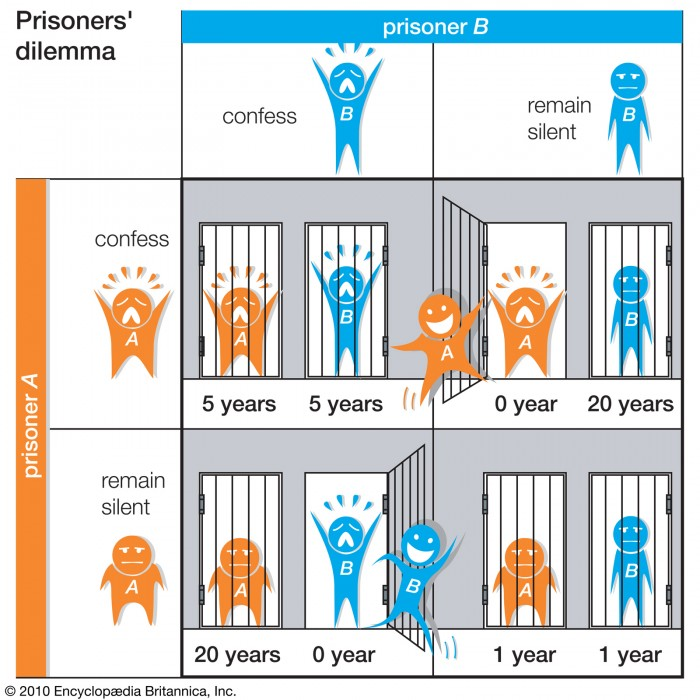
\includegraphics[width=\linewidth]{images/prisoners_dilemma}
	\caption{Fogolydilemma}
\end{figure}
	\end{column}
\end{columns}

\end{frame}


\subsection{Játékelmélet a biológiában}
\begin{frame}
\frametitle{Játékelmélet a biológiában}
\begin{itemize}
	\item evolúciós játékok - játékelmélet alkalmazása populációk alakulásának modellezésére
	\item nem racionális játékosok
	\item fitnesz mint nyereség
	\item evolúciósan stabil stratégia - az azt alkalmazó populáció nem győzhető le semmilyen más, kezdetben kevés létszámú stratégiával
\end{itemize}
\end{frame}

\section{Daganatos sejtek modellezése}
\begin{frame}
\frametitle{Daganatos sejtek modellezése}
\begin{itemize}
	\item daganat - sokszoros mutáció következtében létrejött elburjánzó sejttömörülés
	\item egy daganaton belül többféle sejt $\rightarrow$ agresszívabb sejttípusok megjelenése
\end{itemize}
	\begin{block}{}
	$\Rightarrow$ a játékelmélet egy lehetséges eszköz a sejttípusok közötti versengés modellezésére
\end{block}

\end{frame}

\begin{frame}
	\frametitle{Daganatos sejtek modellezése}
	Lehetséges modellek:
	\begin{itemize}
		\item daganatos sejtek - erőforrásokért folyatott \textbf{verseny}
		\item növekedési faktorokat termelő egészséges sejtek és daganatos sejtek - \textbf{parazitizmus}
		\item immunsejtek - \textbf{ragadozó}
		\item egészséges sejtek, daganatos sejtek - \textbf{mutualizmnus}
	\end{itemize}
\begin{tikzpicture}

\node[anchor=south west,inner sep=0] (image) at (4,0) { 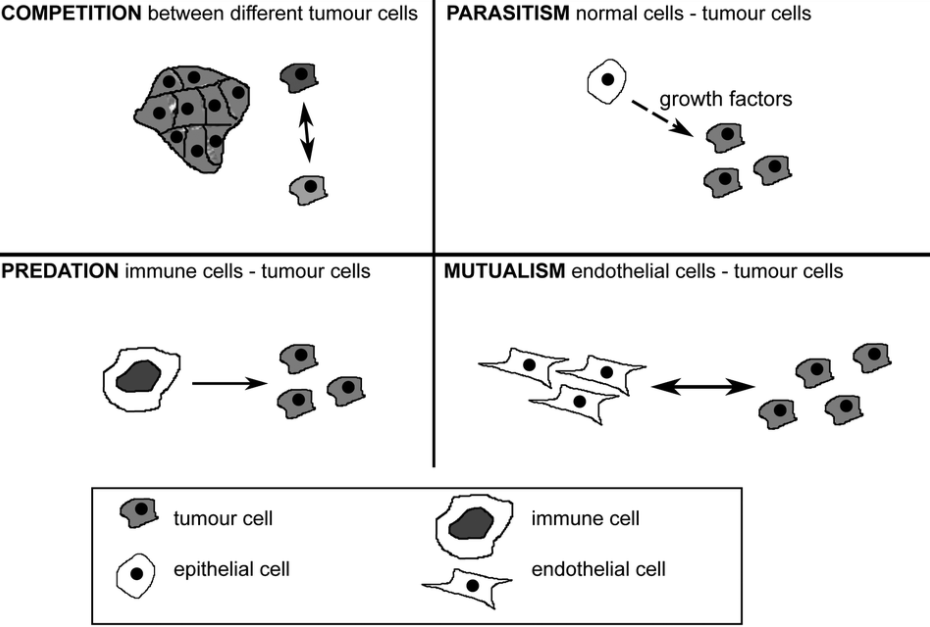
\includegraphics[width=0.5\linewidth]{images/models}};
\pause
\begin{scope}[x={(image.south east)},y={(image.north west)}]
\draw[red,ultra thick,rounded corners] (0.15,0.6) rectangle (0.28,1);
\end{scope}
\end{tikzpicture}

\end{frame}

\subsection{Közjó játék (Public goods game)}
\begin{frame}
\begin{itemize}
	\item növekedési faktorok és jelzőmolekulák szerepe
	\begin{itemize}
		\item saját növekedés elősegítése
		\item a szervezet védekezésének kijátszása
		\item metasztázis kialakulása
	\end{itemize}
	\item ezek az anyagok kikerülhetnek a sejtek közötti térbe
\end{itemize}
\begin{block}
	\centering
	$\Rightarrow$ növekedési faktor mint "közös jó"
\end{block}
\frametitle{Közjó játék (Public goods game)}\end{frame}

\subsection{A játékmodell felépítése}
\subsubsection{Voronoi diagram}
\begin{frame}
	\frametitle{Voronoi diagram}
	\begin{block}{}
		\begin{itemize}
			\item a sejtek ábrázolása Voronoi hálózatokkal
			\item ???szabályos pontrács - figyelmen kívül hagyja a kapcsolatok sokféleségét\cite{archetti2016cooperation}
			\item ??skála-független hálózatok - nem megfelelő, ha az egyedek egy síkban helyezkednek el\cite{archetti2016cooperation}
		\end{itemize}
	\end{block}
	
	\centering
	
\includegraphics[width=0.5\linewidth]{images/Voronoi}
\end{frame}

\subsubsection{A játék szereplői és a stratégiák}
\begin{frame}
	\frametitle{A játék szereplői és a stratégiák}
	A sejtek:
	\begin{itemize}
		\item \textit{kooperálnak} - termelnek növekedési faktorokat
		\item \textit{defektálnak} - nem vesznek részt a faktorok termelésében
	\end{itemize}
	A stratégiák \textit{nyereségének (payoff)} kiszámítása: \(p = b(j) - c\)
	\begin{itemize}
		\item \textit{c} - a növekedési faktor előállításának költsége
		\item \textit{j} - a csoportban résztvevő kooperatív sejtek száma
	\end{itemize}
	ahol 
	\begin{equation}
		b(j) = [V(j) - V(0)]/[V(n) - V(0)]
	\end{equation}
	\begin{equation}
		\label{eq:payoffGradient}
		V(j) = 1/[1 + e^{(-s(j-k)/n)}]
	\end{equation}
\end{frame}

\begin{frame}
	\frametitle{Szabályok}
	\begin{itemize}
		\item véletlenszerűen elhelyezünk defektáló sejteket (arányuk 0.05)
		\item minden körben véletlenszerűen kiválasztunk egy sejtet és annak egy szomszédját 
		\item megvizsgáljuk a nyereségeket
		\item ha a szomszéd stratégiája kifizetődőbb, a kiválasztott sejt átveszi azt
		\item minden kör végén aktualizáljuk a nyereségeket (aszinkron módon számolunk)
	\end{itemize}
\end{frame}

\subsubsection{Diffúziós távolság}
\begin{frame}
	\frametitle{Diffúziós távolság}
	\begin{block}{}
		\begin{itemize}
			\item a diffúziós távolságon belül található összes sejt figyelembe vétele
			\item szomszédok befolyásának súlyozása - diffúziós gradiens
		\end{itemize}
		\begin{equation}
			\label{eq:diffGradient}
			G(i) = [g(i) - g(0)]/[g(D) - g(0)] 
		\end{equation}
		\begin{equation}
			g(i) = 1/[1 + e^{(-z(i-d)/D)}]
		\end{equation}
	\end{block}
	\begin{block}{}
		\begin{itemize}
				\item a termelők száma a \ref{eq:diffGradient}-sal kiszámított súlyozott összeg
		\end{itemize}
	\end{block}
\end{frame}

\subsection{Osztódás}
\begin{frame}
	\frametitle{Osztódás}
	\begin{block}{A Gompertz modell - a tumor méretének időbeli változása}
		\begin{equation}
			n_t = K \bigg(\frac{n_0}{K} \bigg) ^ {e^{(- \alpha t)}},
		\end{equation}
		\begin{itemize}
			\item $n_t$ - a populáció mérete a $t$ időpillanatban
			\item $n_0$ - a populáció kezdeti mérete
			\item $K$ - az elérhető maximális mérete a tumornak
			\item $\alpha$ - egy konstans, a sejtek burjánzási képességével áll összefüggésben
		\end{itemize}
	\end{block}
	\pause
	\begin{block}{}
		\begin{itemize}
			\item az eddigi modellbe könnyen beépíthető
			\item nem veszi figyelembe, hogy éppen milyen típusú sejt (kooperáló/defektáló) osztódik
		\end{itemize}
	\end{block}
\end{frame}
\newcommand{\projectName}{Az EGTIB}

\chapter{\projectName{} bemutatása}

\projectName{} projekt célja egy olyan felhasználóbarát felület létrehozása, mely lehetőséget teremt a daganatos sejtek játékelméleti modellezésére és szimulációjára, valamint a szimulációs eredmények megjelenítésére. Ezért született meg, a mai trendeket figyelembe véve, egy kliens-szerver architektúrán alapuló webalkalmazás, mely részben az \cite{archetti2016cooperation}-ben megjelent modellt implementálja, és ahhoz új funkcionalitásokat is hozzáad.

\begin{figure}[ht!]
	\centering
	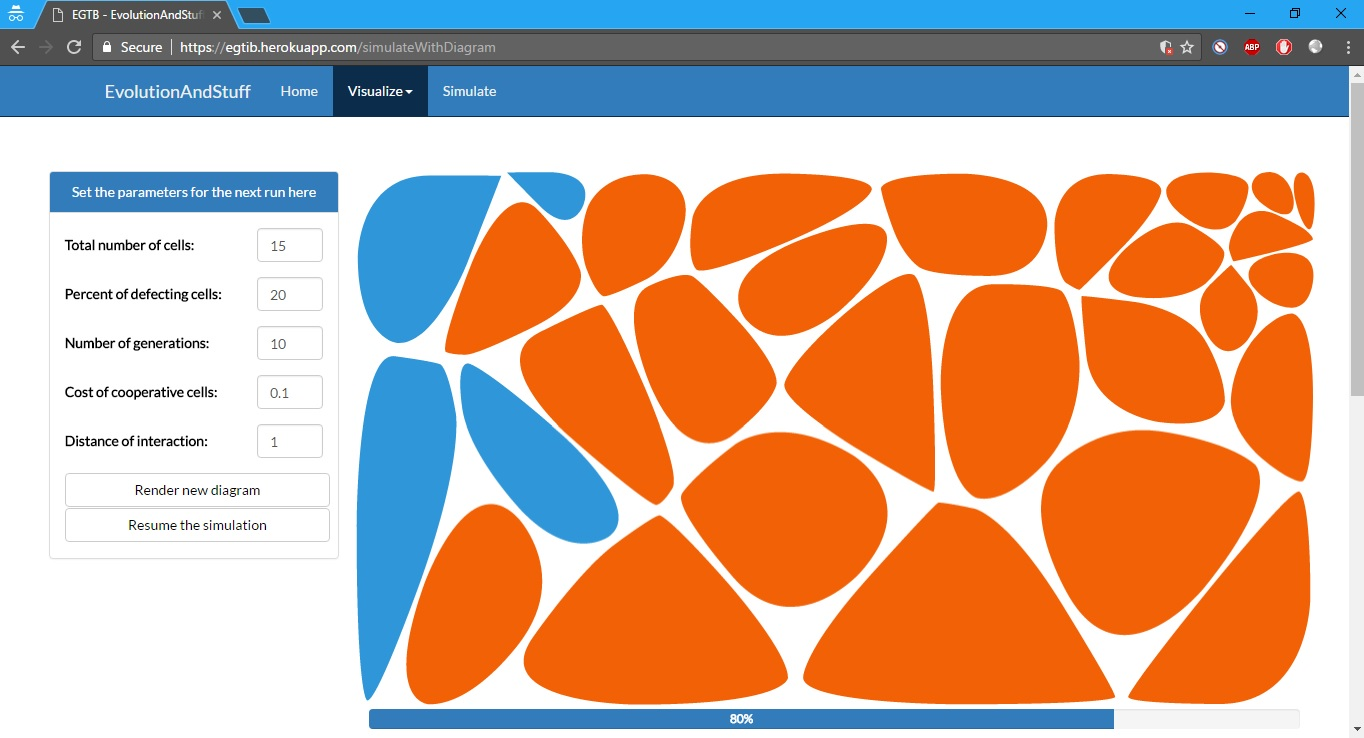
\includegraphics[width=90mm]{images/EGTIB.jpg}
	\caption{Pillanatkép az alkalmazásról \label{fig:SimulateWithDiagram}}
\end{figure}

\section{Funkcionalitások}

A felhasználónak lehetősége van bizonyos paramétereket megválasztani még a szimulálási fázis előtt:
\begin{itemize}[noitemsep]
	\item kezdeti populáció mérete
	\item defektálók aránya 
	\item generáció szám (szimuláció hossza)
	\item kooperáló sejtek termelési költsége 
	\item diffúziós távolság mérete
	\item akarja-e a felhasználó, hogy a sejtek osztódásra legyenek képesek
\end{itemize}
Ezen paramétereket felhasználva kigenerálható egy Voronoi diagram mely a sejteket ábrázolja. A simulate gombot megnyomva ez az adatcsomag eljut a szerverhez amely elvégzi az erőforrás igényes számításokat melynek eredményét visszaküldi a kliensnek, ami majd azt megjeleníti.
Az alkalmazásunkat felhasználási szempontból két fő komponensre oszthatjuk:

\paragraph{Vizualizáció}- képes szimulálni kevés sejtből (max. 500) álló populációkat és ezeket generációnként meg is tudja jeleníteni. A megjelenítés interaktív, ami azt jelenti, hogy bármikor meg lehet állítani, folytatni vagy akár tekergetni mint egy filmet. Továbbá mindehhez tartozik egy grafikon is, mely a populációnak változását ábrázolja generációnként.

\paragraph{Szimuláció}- alkalmas nagyobb (max. 2000) populációval dolgozni, viszont ezek megjelenítése már túl sok időt venne igénybe, így csak a fentebb említett grafikon segítségével ábrázolja azt, hogy mi is történik a sejtek között. Előnye a vizualizációs részhez képest elsősorban az, hogy sokkal nagyobb populációval tud dolgozni, de a paraméterlista is változatosabb (a szimuláció során használt függvények viselkedésébe is bele tud szólni a felhasználó) és hatalmas kényelmi faktornak számít az, hogy több, különböző paraméterezésű szimulációt is képes egy gombnyomással lekérni.

\section{Felhasznált technológiák}

A szoftver egy szerverből és egy kliensből áll, melyek közötti kommunikáció a már jól megszokott HTTP mellett, websocketen keresztül is folyik. Az utóbbira azért van szükség, mert gyorsítja az adatok áramlását, és alkalmas nagyobb mennyiségű adat átvitelére, mely a szimuláció során keletkezik. 

Kliens oldali technológiák közé sorolandó a Bootstrap \cite{soft:bootstrap}, mely segítségével nem csak desktopon de mobil platformon is elegáns az oldal kinézete, valamint az AngularJS \cite{soft:angular}, ami biztosítja az oldal dinamikusságát. A Paper.js \cite{soft:paper} a rajzok megjelenítéséért felelős, és ennek egy segédkönyvtára \cite{soft:voronoiModule} pedig kifejezetten a voronoi diagram ábrázolásáért, úgy vizuálisan mint adatszerkezeti szinten is. A grafikonok kirajzolását kezdetben a Highchartsra \cite{soft:highcharts} míg a későbbiekben a könnyebben használható Plotly.js-re \cite{soft:plotly} bíztuk.

A szerverünk NodeJS \cite{soft:node} alapú, az Express \cite{soft:express} keretrendszert használja fel. Itt folyik az erőforrás igényes számítások nagy része, így itt is jelen van a Paper.js voronoi modulja \cite{soft:voronoiModule}.

Mindezt összefogva és belerakva egy Dockerbe \cite{soft:docker}, már mehet is egy felhőbe, a mi esetünkben ez a Heroku (https://egtib.herokuapp.com/). A fejlesztési és tesztelési folyamatot amennyire csak lehetett megpróbáltuk automatizálni, így a Travis CI \cite{soft:travis} az, ami a projektünket teszteli és amennyiben szükséges kitelepíti a legújabb verziót a felhőbe.

Az alkalmazásunk minőségét unit és E2E tesztekkel próbáltuk meg biztosítani, ezekhez a Mocha \cite{soft:mocha} és TestCafe \cite{soft:testcafe} keretrendszereket használtuk.

\begin{figure}[ht!]
	\centering
	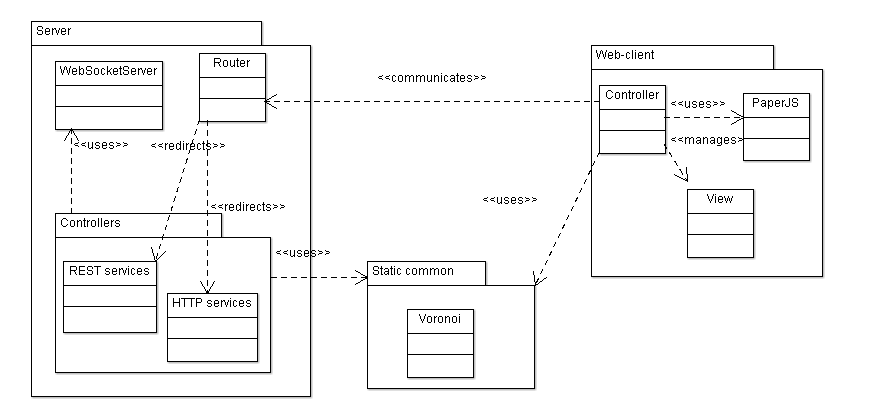
\includegraphics[width=\linewidth]{images/Architecture}
	\caption{A projekt architektúrája\label{fig:Architecture}}
\end{figure}

\section{A szimuláció eredményei}
\begin{frame}
	\frametitle{A szimuláció eredményei}
	\begin{block}{Adatok összevetése}
		A már rendelkezésünkre álló bemeneti paraméterekre\cite{archetti2016cooperation} elvégeztünk 100-100 szimulációt, minden egyes diffúziós távolságra 1-től 5-ig.
	\end{block}

	\begin{block}{Paraméterek}
		\begin{multicols}{2}
			\begin{itemize}
				\item populáció mérete: 1000
				\item defektálók: 5\%
				\item generációk száma: 15
				\item kooperálók költsége: 0.01
				\item osztódás: nincs
			\end{itemize}
			\begin{itemize}
				\item $s = 2$
				\item $k = 1$
				\item $d = \frac{1}{2}D$
				\item $z = 20$
			\end{itemize}	
		\end{multicols}
	\end{block}
\end{frame}

\begin{frame}
	\frametitle{Összehasonlítás}
	\begin{figure}[h]
		\centering
		\begin{tabular}{cc}
			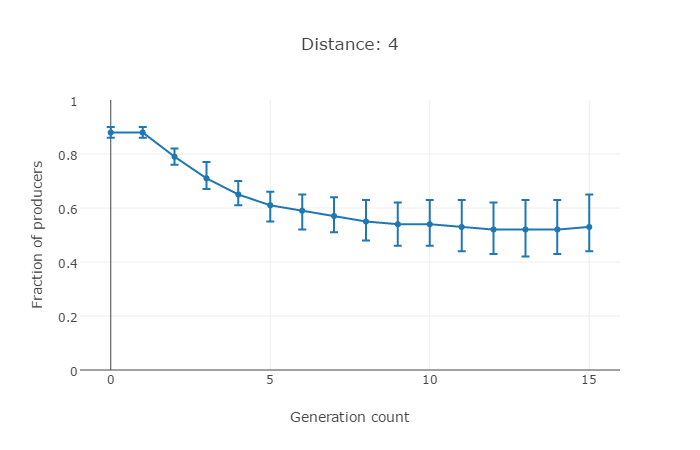
\includegraphics[width=0.4\linewidth]{images/dist4}
			&
			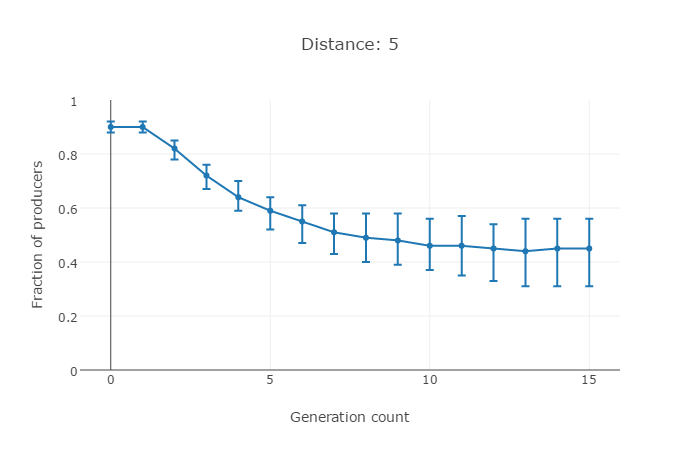
\includegraphics[width=0.4\linewidth]{images/dist5}
			\\
			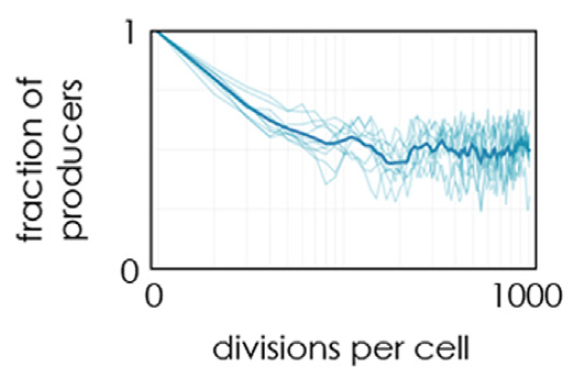
\includegraphics[width=0.4\linewidth]{images/arc_dist4}
			&
			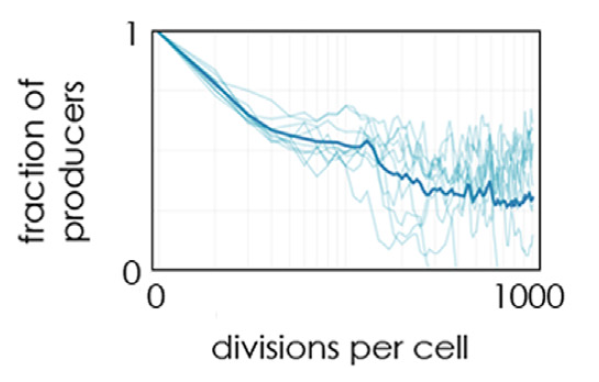
\includegraphics[width=0.4\linewidth]{images/arc_dist5}
			\\
		\end{tabular}
		\caption{Szimulációs eredmények a fenti paraméterekre és azok párjai a \cite{archetti2016cooperation} cikkből}
		\label{fig:DistChange}
	\end{figure}
\end{frame}

\subsection{A költség és nyereség hatása}
\begin{frame}
	\frametitle{A költség és nyereség hatása}
	\begin{block}{}
			\begin{itemize}
				\item sokba kerül a termelés $\Rightarrow$ megéri élősködni
				\item alacsony költség $\Rightarrow$ fenntartható egy bizonyos egyensúly
			\end{itemize}
	\end{block}

	\begin{figure}[h]
		\centering
		\begin{tabular}{cc}
			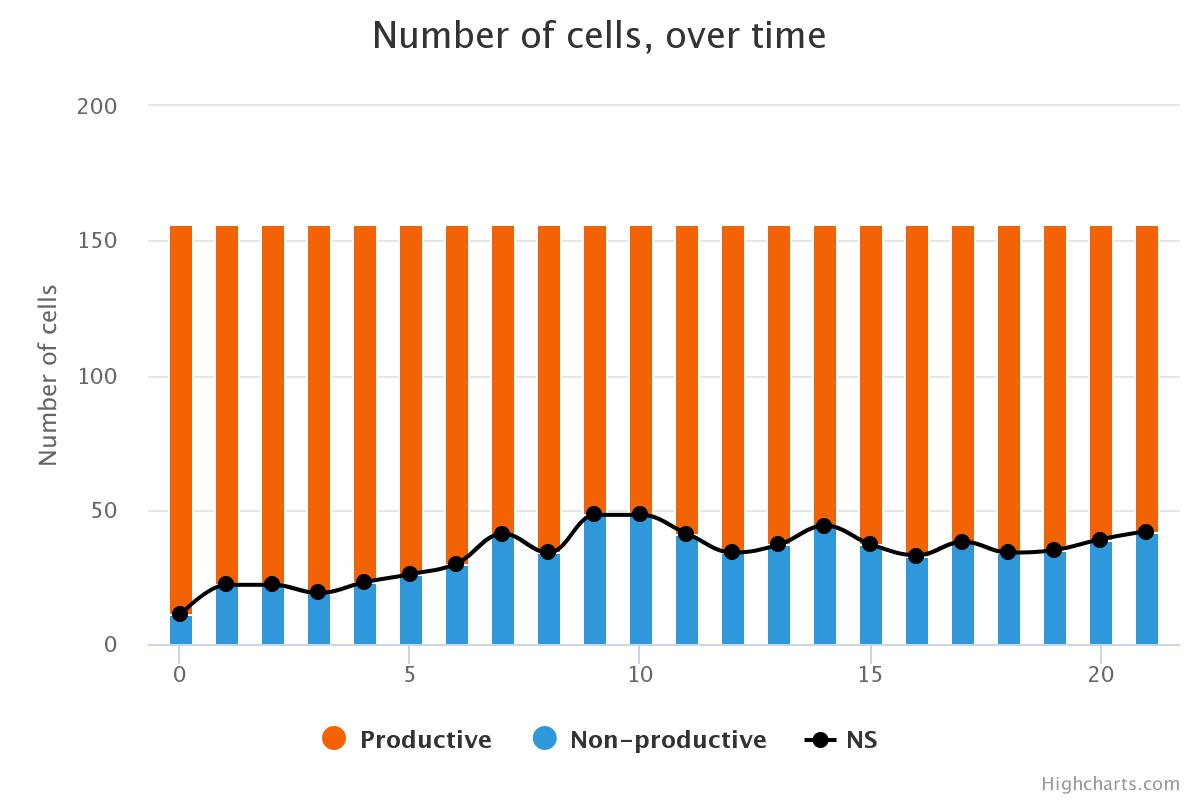
\includegraphics[width=0.35\linewidth]{images/chart001.jpeg}
			&
			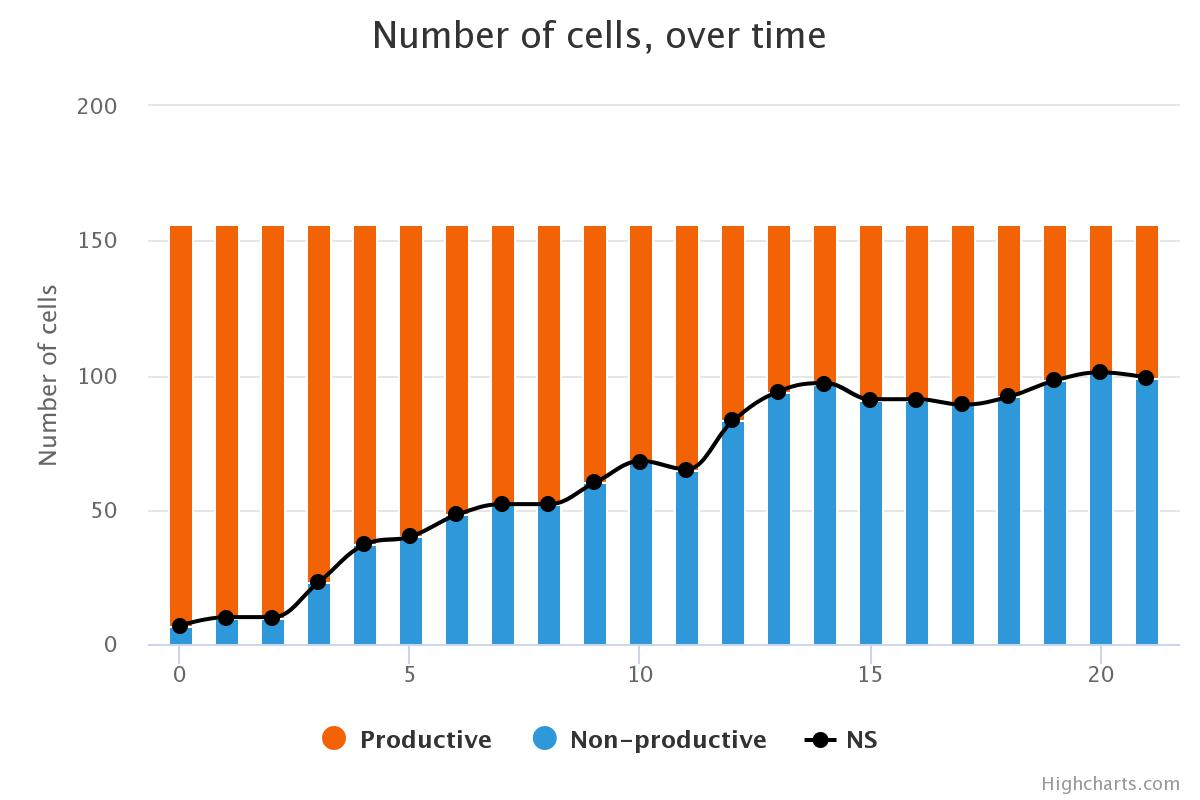
\includegraphics[width=0.35\linewidth]{images/chart01.jpeg}
		\end{tabular}
		\begin{tabular}{cl}  
			\begin{tabular}{c}
				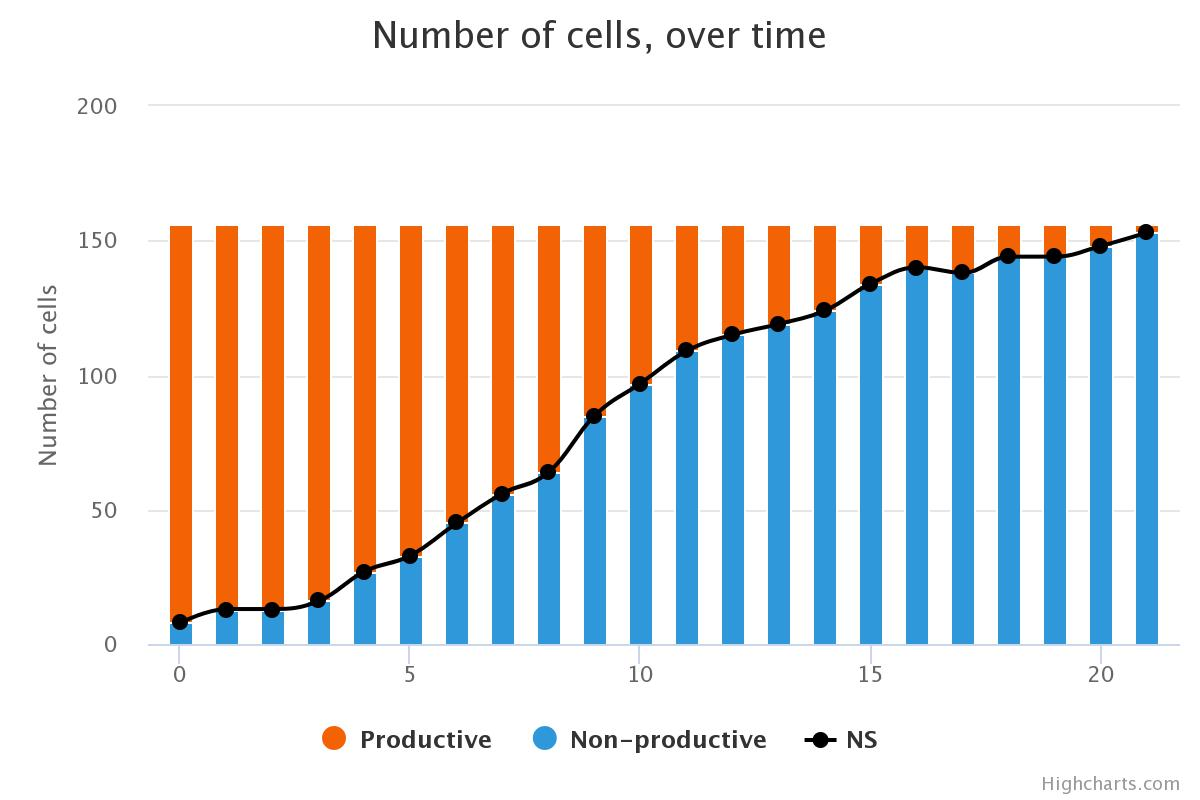
\includegraphics[width=0.35\linewidth]{images/chart08.jpeg}
			\end{tabular}
			& 
			\begin{tabular}{l}
				\parbox{0.35\linewidth}{
					A játék végkimenetele mikor a költségek rendre 0.01, 0.1 és 0.8
				}
			\end{tabular}  \\
		\end{tabular}
		\label{fig:CoopCostChange}
	\end{figure}
\end{frame}

\subsection{Diffúziós távolság hatása}
\begin{frame}
	\frametitle{Diffúziós távolság hatása}
	\begin{itemize}
		\item a diffúziós távolság növelésével valósághűbb adatokat kaphatunk
		\item a távolság növekedésével a defektáló sejtek könnyebben terjednek
		\item ezt a paramétert a hasnyálmirigyrák esetén megállapították\cite{archetti2015heterogeneity}
	\item az esetek túlnyomó részében ez az érték 5-10-től 30-60-ig terjedhet\cite{archetti2016cooperation}
	\end{itemize}
	
	\begin{figure}[h]
		\centering
		\begin{tabular}{cc}
			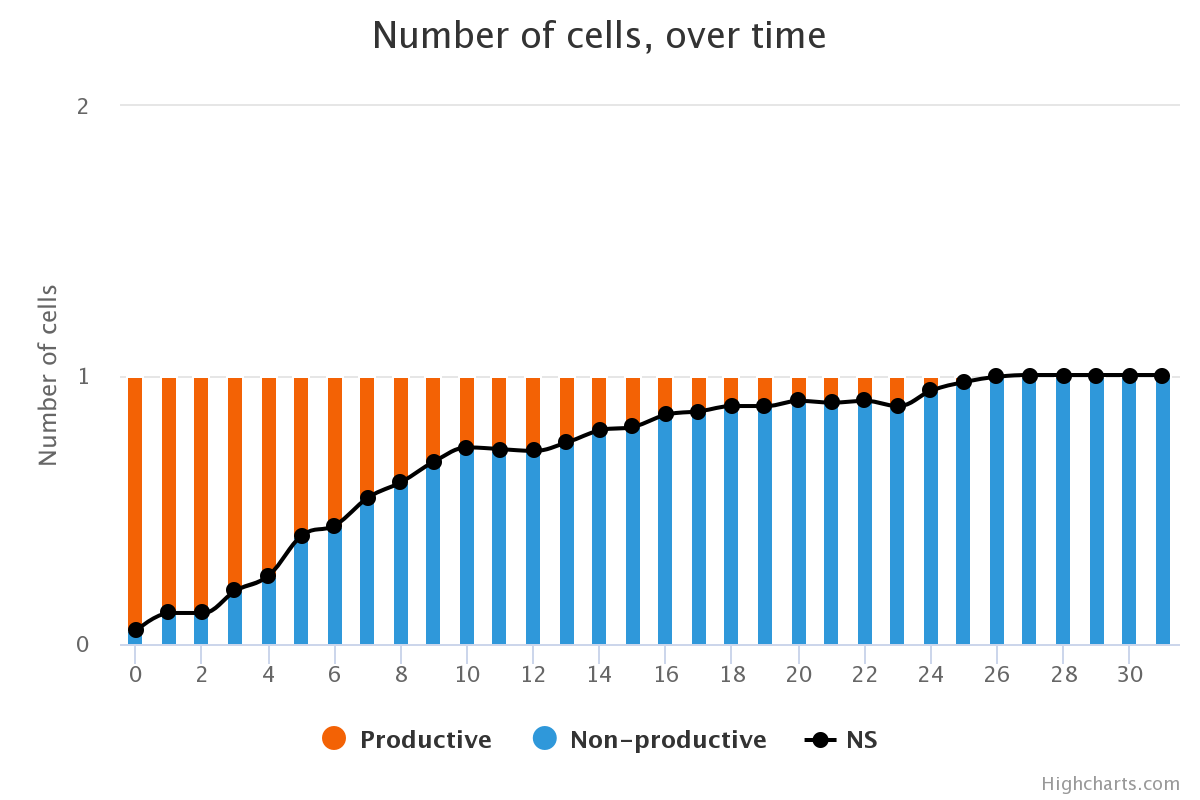
\includegraphics[width=0.4\linewidth]{images/diffdist2}
			&
			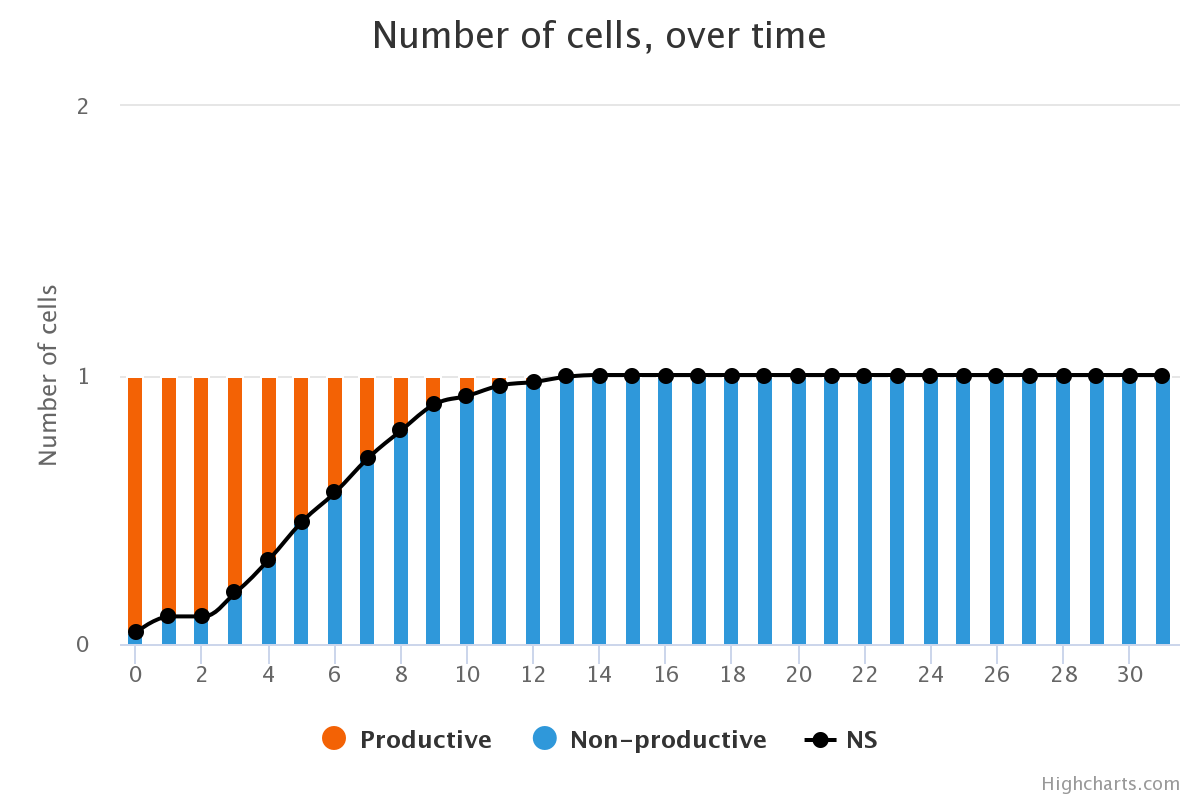
\includegraphics[width=0.4\linewidth]{images/diffdist5}
		\end{tabular}
		\caption{A játék végkimenetele két diffúziós távolságra. A paraméterek: 160 sejt, 5\% defektáló, 0.3 költség, távolság: 2 illetve 5}
		\label{fig:DiffDist}
	\end{figure}
\end{frame}

\subsection{Osztódásra képes populációk}
\begin{frame}
	\frametitle{Osztódásra képes populációk}
	\begin{itemize}
		\item eddigi a populáció mérete állandó volt és egy adott modellt követett
		\item a valóságban a defektáló sejtek nem csak területileg terjednek el
		\item számosságban is túlnövik a kooperálókat
	\end{itemize}
	
	\begin{columns}
		\column{0.5\textwidth}
			\begin{figure}[ht]
				\centering
				\begin{tabular}{c}
					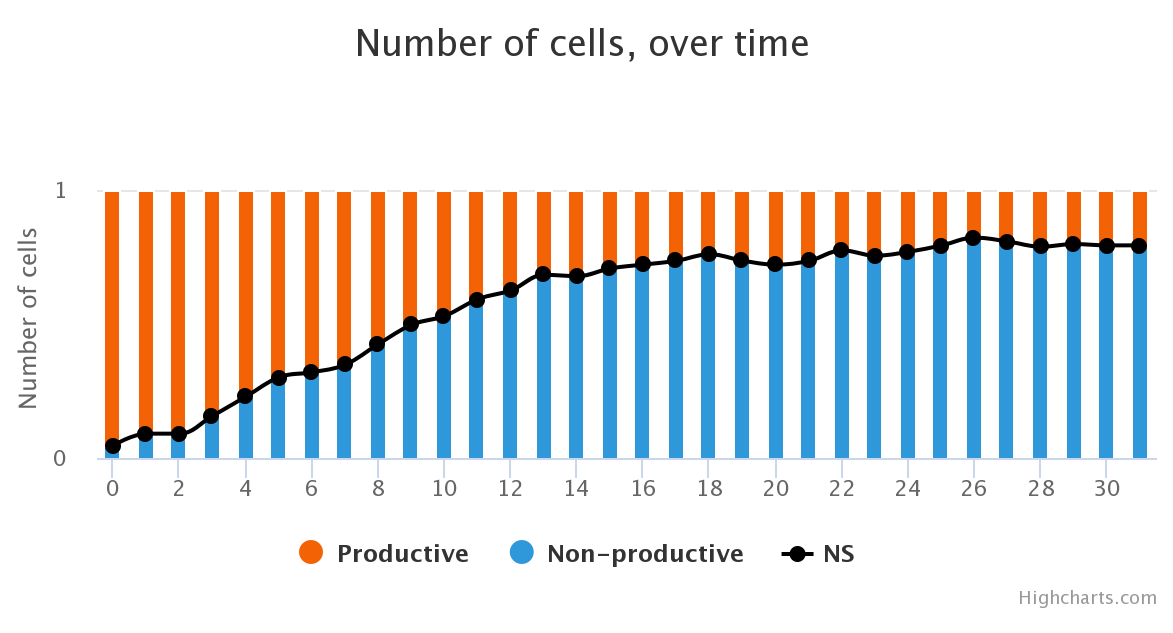
\includegraphics[width=0.9\textwidth]{images/nemosztodik}
					\\
					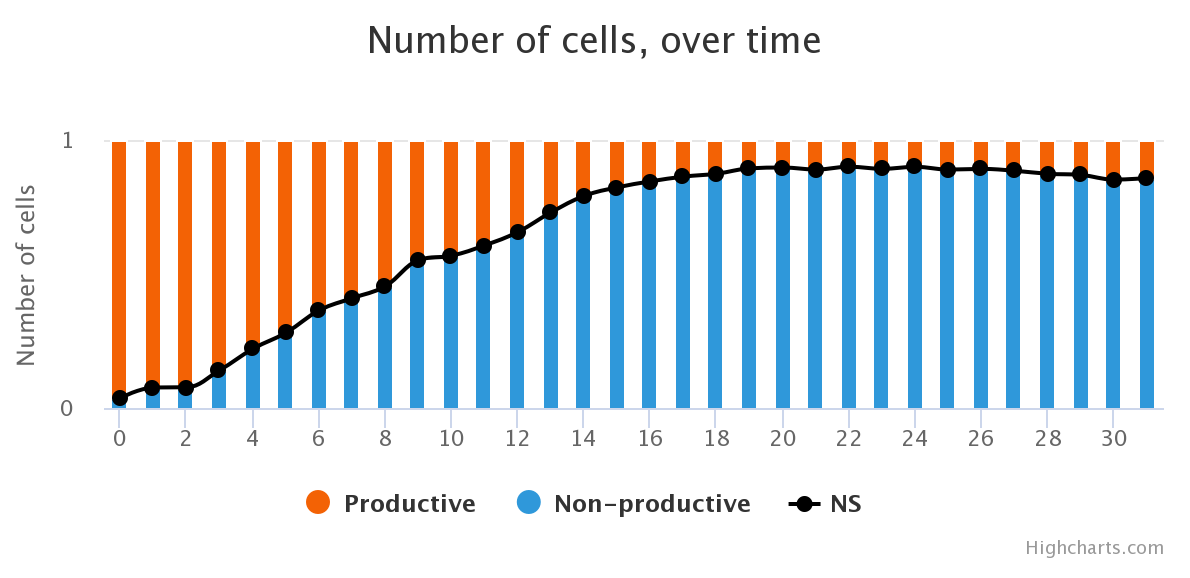
\includegraphics[width=0.9\textwidth]{images/osztodik}
				\end{tabular}
				\caption{Az első esetben a sejtek nem osztódtak míg a másodikban igen}				\label{fig:Divide}
			\end{figure}
		\column{0.5\textwidth}
			\begin{block}{}
				\begin{itemize}
					\item az új sejtek képesek felgyorsítani a defektálók terjedését
					\item további kísérletek szükségesek
				\end{itemize}
			\end{block}
	\end{columns}
\end{frame}

\begin{frame}
	\frametitle{Osztódással vagy anélkül?}
	\begin{table}
		\caption{Osztódás nélküli modell}
		\label{table:nemOsztodik}
		\adjustbox{max height=\dimexpr\textheight-5.5cm\relax, max width=\textwidth}{
			\begin{tabular}{ | l | l | l | l | l | l | l | l | l | l | l | l | }
				\hline
				\multirow{3}{*}{D = 2}
				& Generáció & 1 & 2 & 3 & 4 & 5 & 6 & 7 & 8 & 9 & 10 \\ \cline{2-12}
				& CoopPerc & 0.91 & 0.91 & 0.85 & 0.81 & 0.77 & 0.75 & 0.73 & 0.71 & 0.69 & 0.68 \\ \cline{2-12}
				& stdev & 0.01 & 0.01 & 0.02 & 0.03 & 0.03 & 0.03 & 0.05 & 0.05 & 0.05 & 0.06 \\ \hline
				\multirow{3}{*}{D = 3}
				& Generáció & 1 & 2 & 3 & 4 & 5 & 6 & 7 & 8 & 9 & 10 \\ \cline{2-12}
				& CoopPerc & 0.9 & 0.9 & 0.83 & 0.77 & 0.72 & 0.68 & 0.66 & 0.64 & 0.62 & 0.6 \\ \cline{2-12}
				& stdev & 0.02 & 0.02 & 0.03 & 0.04 & 0.04 & 0.05 & 0.04 & 0.05 & 0.05 & 0.04 \\ \hline
			\end{tabular}
		}
	\end{table}
	
	\begin{table}
		\caption{Osztódást használó modell}
		\label{table:osztodik}
		\adjustbox{max height=\dimexpr\textheight-5.5cm\relax, max width=\textwidth}{
			\begin{tabular}{ | l | l | l | l | l | l | l | l | l | l | l | l | }
				\hline
				\multirow{3}{*}{D = 2}
				& Generáció & 1 & 2 & 3 & 4 & 5 & 6 & 7 & 8 & 9 & 10 \\ \cline{2-12}
				& CoopPerc & 0.87 & 0.87 & 0.79 & 0.74 & 0.7 & 0.67 & 0.64 & 0.61 & 0.59 & 0.57 \\ \cline{2-12}
				& stdev & 0.02 & 0.02 & 0.03 & 0.04 & 0.05 & 0.06 & 0.07 & 0.05 & 0.07 & 0.07 \\ \hline
				\multirow{3}{*}{D = 3}
				& Generáció & 1 & 2 & 3 & 4 & 5 & 6 & 7 & 8 & 9 & 10 \\ \cline{2-12}
				& CoopPerc & 0.89 & 0.9 & 0.82 & 0.75 & 0.7 & 0.66 & 0.62 & 0.59 & 0.56 & 0.54 \\ \cline{2-12}
				& stdev & 0.03 & 0.04 & 0.05 & 0.06 & 0.08 & 0.08 & 0.08 & 0.09 & 0.09 & 0.09 \\ \hline
			\end{tabular}
		}
	\end{table}
\end{frame}

\section{Összegzés}

Elmondhatjuk, hogy sikerült egy olyan szoftvert létrehoznunk mely segítségével jobban megérhetjük, hogy mi is történik egy daganaton belül. Fő erőssége a kísérletezésben rejlik, de kutatási vagy akár tanítási célokra is fel lehet használni.

Természetesen hiányosságai is vannak, melyeket a jövőben szeretnénk pótolni. Rendkívül hasznos lenne azon funkció mely során egy terápiát alkalmazunk, vagy ellenanyagokat juttatunk be, melyek a termelést, annak költségét befolyásolják. Komoly kihívásnak számít az, hogy különböző ráktípusokra meghatározzuk az őket leíró paramétereket. A számítások hatékonyságágának növelése is egy fontos feladat, ami maga után vonná azt a tényt, hogy nagyobb populációkkal is szimulálhatunk. 

Az általunk végzett szimulációk arra a feltételezésre engednek következtetni, hogy a sejtek játéka bizonyos határokon belül leírja a daganatok viselkedését és hisszük azt, hogy a játékelmélettel ezen területet ki lehet aknázni.

\bibliography{articles}
\bibliographystyle{ieeetr}
\end{document}